\documentclass[12pt]{article}

\usepackage{amssymb,amsmath,amsthm}
\usepackage[top=1in, bottom=1in, left=1.25in, right=1.25in]{geometry}
\usepackage{fancyhdr}
\usepackage{enumerate}
\usepackage[bw,framed,numbered]{mcode}
\usepackage{graphicx}

% Comment the following line to use TeX's default font of Computer Modern.
\usepackage{times,txfonts}

\newtheoremstyle{homework}% name of the style to be used
  {18pt}% measure of space to leave above the theorem. E.g.: 3pt
  {12pt}% measure of space to leave below the theorem. E.g.: 3pt
  {}% name of font to use in the body of the theorem
  {}% measure of space to indent
  {\bfseries}% name of head font
  {:}% punctuation between head and body
  {2ex}% space after theorem head; " " = normal interword space
  {}% Manually specify head
\theoremstyle{homework} 

% Set up an Exercise environment and a Solution label.
\newtheorem*{exercisecore}{Exercise \@currentlabel}
\newenvironment{exercise}[1]
{\def\@currentlabel{#1}\exercisecore}
{\endexercisecore}

\newcommand{\localhead}[1]{\par\smallskip\noindent\textbf{#1}\nobreak\\}%
\newcommand\solution{\localhead{Solution:}}

%%%%%%%%%%%%%%%%%%%%%%%%%%%%%%%%%%%%%%%%%%%%%%%%%%%%%%%%%%%%%%%%%%%%%%%%
%
% Stuff for getting the name/document date/title across the header
\makeatletter
\RequirePackage{fancyhdr}
\pagestyle{fancy}
\fancyfoot[C]{\ifnum \value{page} > 1\relax\thepage\fi}
\fancyhead[L]{\ifx\@doclabel\@empty\else\@doclabel\fi}
\fancyhead[C]{\ifx\@docdate\@empty\else\@docdate\fi}
\fancyhead[R]{\ifx\@docauthor\@empty\else\@docauthor\fi}
\headheight 15pt

\def\doclabel#1{\gdef\@doclabel{#1}}
\doclabel{Use {\tt\textbackslash doclabel\{MY LABEL\}}.}
\def\docdate#1{\gdef\@docdate{#1}}
\docdate{Use {\tt\textbackslash docdate\{MY DATE\}}.}
\def\docauthor#1{\gdef\@docauthor{#1}}
\docauthor{Use {\tt\textbackslash docauthor\{MY NAME\}}.}
\makeatother

% Shortcuts for blackboard bold number sets (reals, integers, etc.)
\newcommand{\Reals}{\ensuremath{\mathbb R}}
\newcommand{\Nats}{\ensuremath{\mathbb N}}
\newcommand{\Ints}{\ensuremath{\mathbb Z}}
\newcommand{\Rats}{\ensuremath{\mathbb Q}}
\newcommand{\Cplx}{\ensuremath{\mathbb C}}
%% Some equivalents that some people may prefer.
\let\RR\Reals
\let\NN\Nats
\let\II\Ints
\let\CC\Cplx

%%%%%%%%%%%%%%%%%%%%%%%%%%%%%%%%%%%%%%%%%%%%%%%%%%%%%%%%%%%%%%%%%%%%%%%%%%%%%%%%%%%%%%%
%%%%%%%%%%%%%%%%%%%%%%%%%%%%%%%%%%%%%%%%%%%%%%%%%%%%%%%%%%%%%%%%%%%%%%%%%%%%%%%%%%%%%%%
% 
% The main document start here.

% The following commands set up the material that appears in the header.

%%%%%%%%%%%%%%%%%%%%%%%%%%%%%%%%%%%%%%%%%%%%%%%%%%%%%%%%%%%%%%%%%%%%%%%%%%%%%%%%%%%%%%%
%%%%%%%%%%%%%%%%%%%%%%%%%%%%%%%%%%%%%%%%%%%%%%%%%%%%%%%%%%%%%%%%%%%%%%%%%%%%%%%%%%%%%%%
% 
% The main document start here.

% The following commands set up the material that appears in the header.
\doclabel{Math 310: Homework 12}
\docauthor{Parker Whaley}
\docdate{December 9, 2016}

\newcommand{\vv}{\mathbf{v}}
\begin{document}
\begin{exercise}
1
Problem 9.6
\end{exercise}
Note that the Taylor estimation is $f(x+c)= f(x) + f'(x)c+ f''(x)c^2/2+f'''(x)c^3/6+O(c^4)$.  We are asked to find the values of the constants in the equation $f''(x)\approx Af(x)+Bf(x+h)+Cf(x+2h)$ that give the maximal accuracy in terms of the magnitude of $h$.  Note that using Taylor's approximation we get $f''(x)\approx Af(x)+B[f(x) + f'(x)h+ f''(x)h^2/2+f'''(x)h^3/6]+C[f(x) + 2f'(x)h+ 2f''(x)h^2+4f'''(x)h^3/3]+O(h^4)$.  We then get the equations $A+B+C=0$ to link values, $Bh+2Ch=0$, $Bh^2/2+2Ch^2=1$.  Solving we get $-B=2C$, $Bh^2/2-Bh^2=1$, $Bh^2(1/2-1)=-Bh^2/2=1$, $B=-2/h^2$, $C=1/h^2$, $A=1/h^2$.  To determine order accuracy let's ask if we also happen to get $0f'''(x)$, $Bh^3/6+C4h^3/3=0$, $B+8C=0$, clearly false, thus we get error of order $O(h^3/h^2)=O(h)$.
\begin{exercise}
2
Turn in the last problem from the worksheet on Richardson extrapolation.
\end{exercise}
\lstinputlisting{../octave/traprule.m}
\lstinputlisting{../octave/q2.m}
This is a plot of the $Ik(N)$ lines for $k=[0:3]$ notice that there slopes are $-2,-4,-6,-8$ indicating that the error goes as $O(n^{-2}),O(n^{-4}),O(n^{-6}),O(n^{-8})$.\\
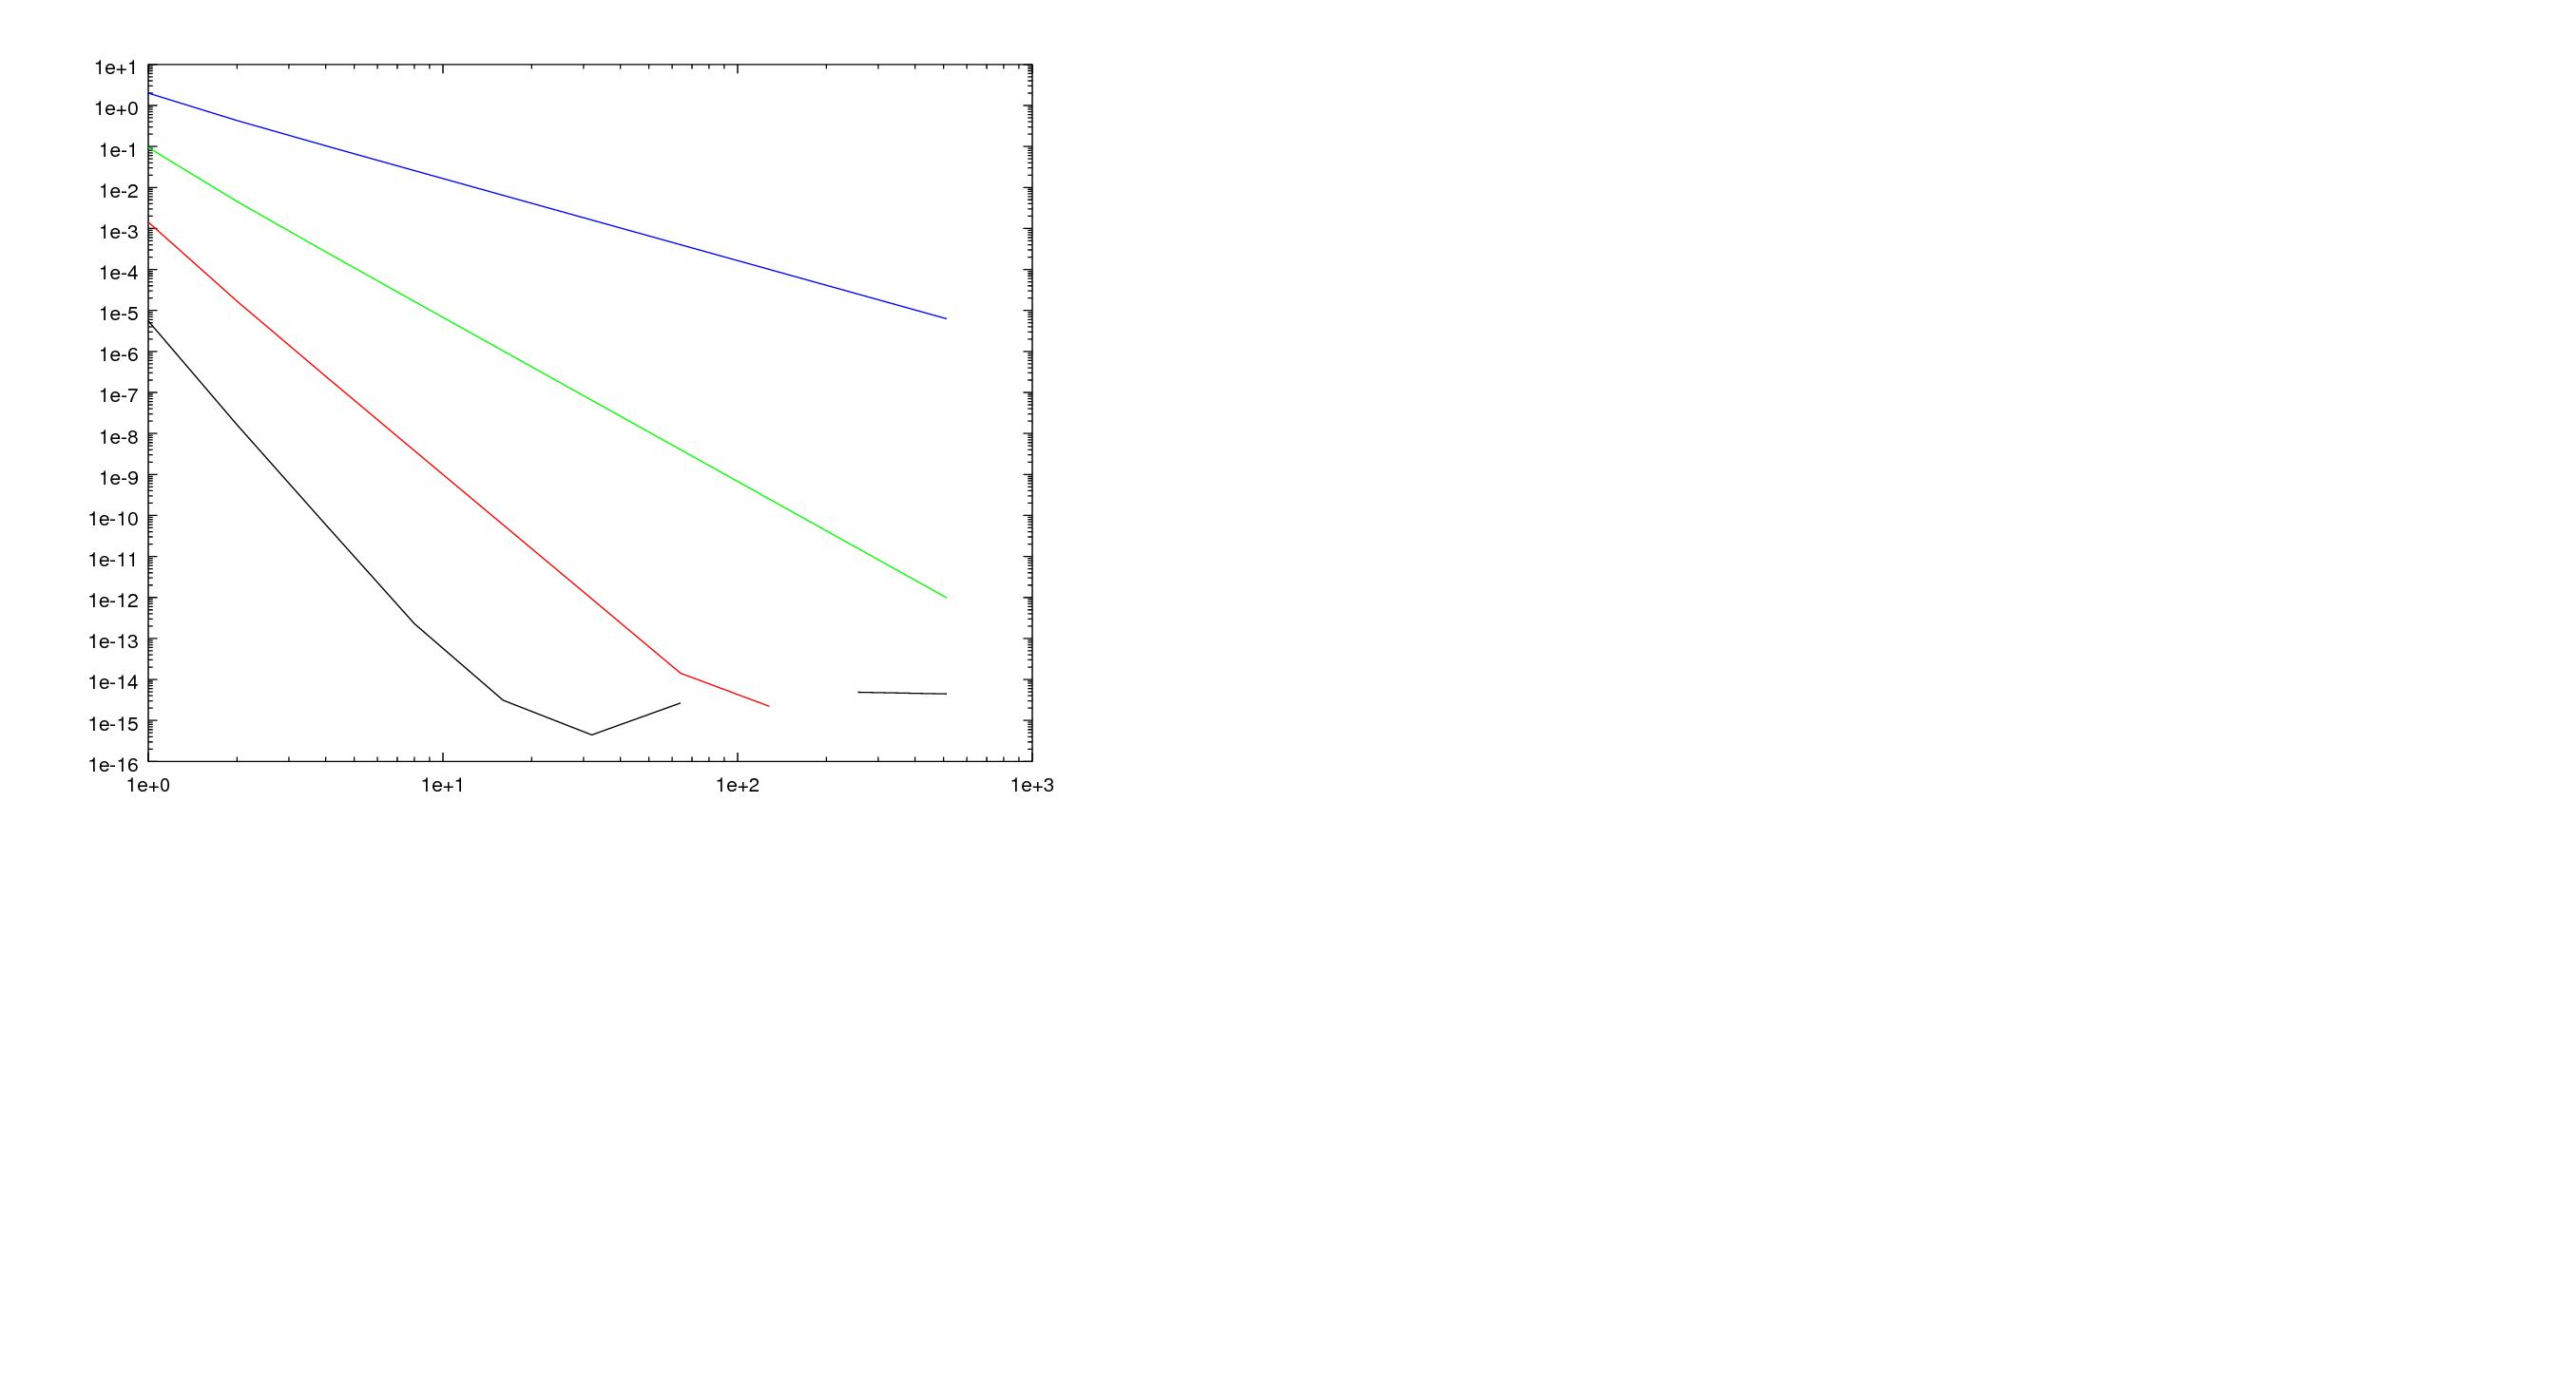
\includegraphics[scale=.6]{../octave/f1.jpg}
\begin{exercise}
3
Problem 10.8. Note that Romberg integration is just Richardson extrapolation applied to the trapezoidal rule, as you did in the previous problem.
\end{exercise}
\lstinputlisting{../octave/d1.txt}
The trapezoidal rule will take around $300,000$ steps to achieve the desired accuracy.  This is because the error in the trapezoid rule goes as $O(n^2)$ where as the Romberg integration is just Richardson extrapolation and increases the order of convergence as the number of steps increases.
\begin{exercise}
4
Problem 11.1 (a,b)
\end{exercise}
Solve analytically
\begin{enumerate}[(a)]
\item
$$\frac{dy}{dt}=t^3$$
$$y=\int dy=\int t^3dt=t^4/4+C$$
$$y=t^4/4$$
\item
$$\frac{dy}{dt}=2y$$
$$\int \frac{1}{y} dy=\int 2 dt$$
$$\ln (y)=2t+c$$
$$\ln (3)=2+c$$
$$\ln (y)=2t+\ln (3)-2$$
\item
$$\frac{dy}{dt}=ay+b$$
$$\text{Ansatz: } y=ce^{\alpha t}+\beta$$
$$\alpha ce^{\alpha t} =ace^{\alpha t}+a\beta+b$$
$$\alpha=a\text{ and } \beta=-b/a$$
$$y=ce^{a t}-b/a$$
$$y_0=ce^{a 0}-b/a$$
$$y=(y_0+b/a)e^{a t}-b/a$$
\end{enumerate}

\begin{exercise}
5
Problem 11.3
\end{exercise}
If $y=t^{3/2}$ then $y'=3/2t^{1/2}$.  Noting that $t^{1/2}=y^{1/3}$ we see $y'=3/2y^{1/3}$ and note that $(0,0)$ is a solution to $y=t^{3/2}$.  Clearly $y=t^{3/2}$ is a solution to the given ODE.  As a demonstration I will use one step of euler method on this problem.  Note that $y_1=0+0*h$ and $t_1=h$.  By inspection Euler method will give us $y=0$ always.  Note that $y=0$ is actually a solution to the given ODE and initial conditions, this is the problem, there are multiple solutions to the ODE passing through $(0,0)$.

\begin{exercise}
6
Problem 11.4
\end{exercise}
\lstinputlisting{../octave/d2.txt}
\begin{exercise}
7
Problem 11.6
\end{exercise}
For $y'(y)=\lambda y$ we know that the slopes needed for RK4 will be 
$$s_1=y'(y_k)=\lambda y_k$$
$$s_2=y'(y_k+s_1*h/2)=\lambda (y_k+\lambda y_k*h/2)=\lambda y_k+\lambda^2 y_k*h/2$$
$$s_3=y'(y_k+s_2*h/2)=\lambda (y_k+(\lambda y_k+\lambda^2 y_k*h/2)*h/2)=\lambda y_k+\lambda^2 y_k*h/2+\lambda^3 y_k*(h/2)^2$$
$$s_4=y'(y_k+s_3*h)=\lambda (y_k+s_3*h)=\lambda y_k+\lambda^2 y_kh+\lambda^3 y_k*h^2/2+\lambda^4 y_k*h^3/4$$
$$y_{k+1}=y_k+h/6(s_1+2s_2+2s_3+s_4)=y_k+h/6(6\lambda y_k+3\lambda^2 y_k*h+\lambda^3 y_k*h^2+\lambda^4 y_k*h^3/4)=$$
$$[1+\lambda h +\lambda^2 h^2/2+\lambda^3 h^3/6+\lambda^4 h^4/24)]y_k$$
\begin{exercise}
8
Problem 11.14 (a,b)
\end{exercise}
\begin{enumerate}[(a)]
\item
The new system of equations would be 
$$\begin{bmatrix}
x'\\
y'\\
z'\\
w'
\end{bmatrix}
=
\begin{bmatrix}
z\\
w\\
\frac{-x}{(x^2+y^2)^{2/3}}\\
\frac{-y}{(x^2+y^2)^{2/3}}
\end{bmatrix}$$
\item
This is my general orbit evaluater
\lstinputlisting{../octave/orbit.m}
and here are euler and RK4
\lstinputlisting{../octave/euler.m}
\lstinputlisting{../octave/RK4.m}
here is the evaluation
\lstinputlisting{../octave/d3.txt}
and the figures\\
\begin{tabular}{c c}
euler & RK4\\
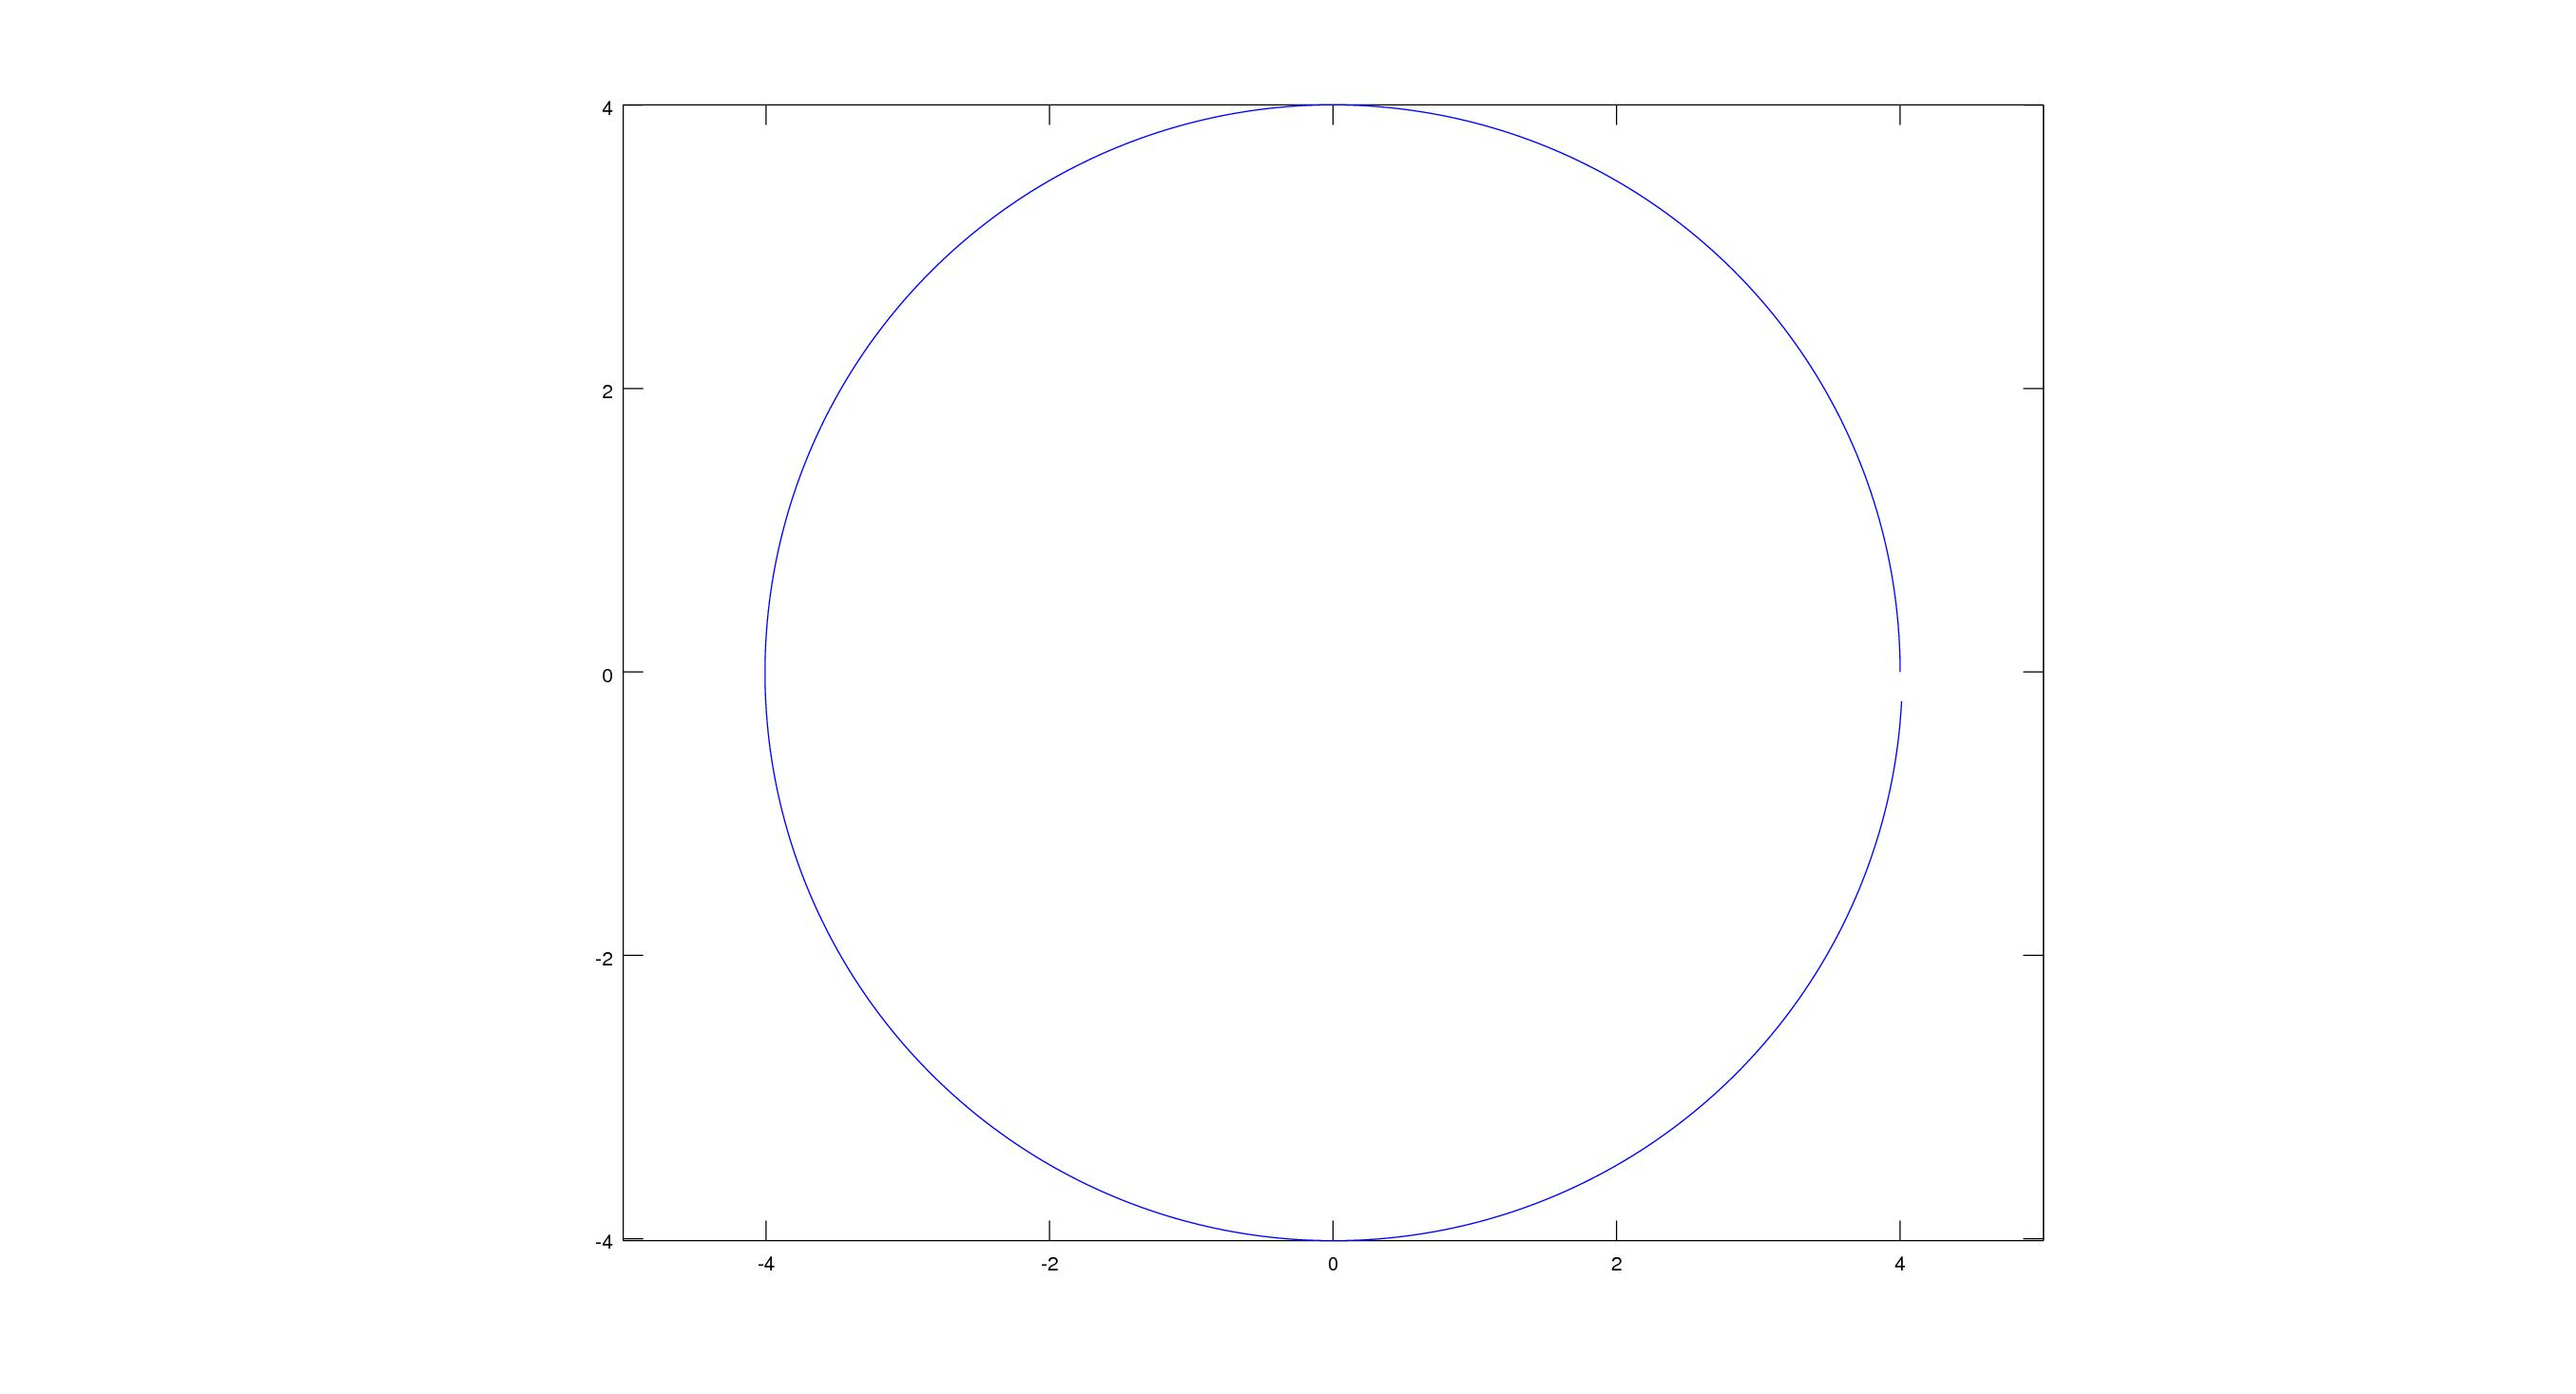
\includegraphics[scale=.15]{../octave/f2.jpg} & 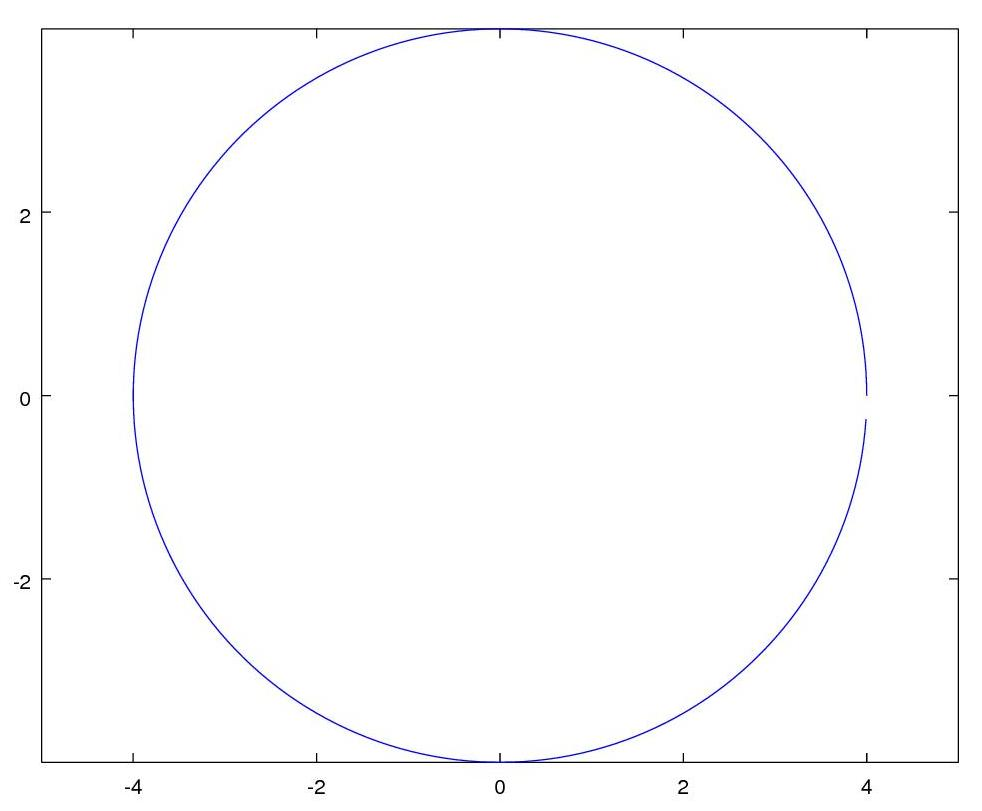
\includegraphics[scale=.3]{../octave/f3.jpg}
\end{tabular}\\
And here are the requested runs notation is [w(0),h,tmax]\\
\begin{tabular}{c c}
$[0.5,0.25,50]$ & $[0.6,0.5,150]$\\
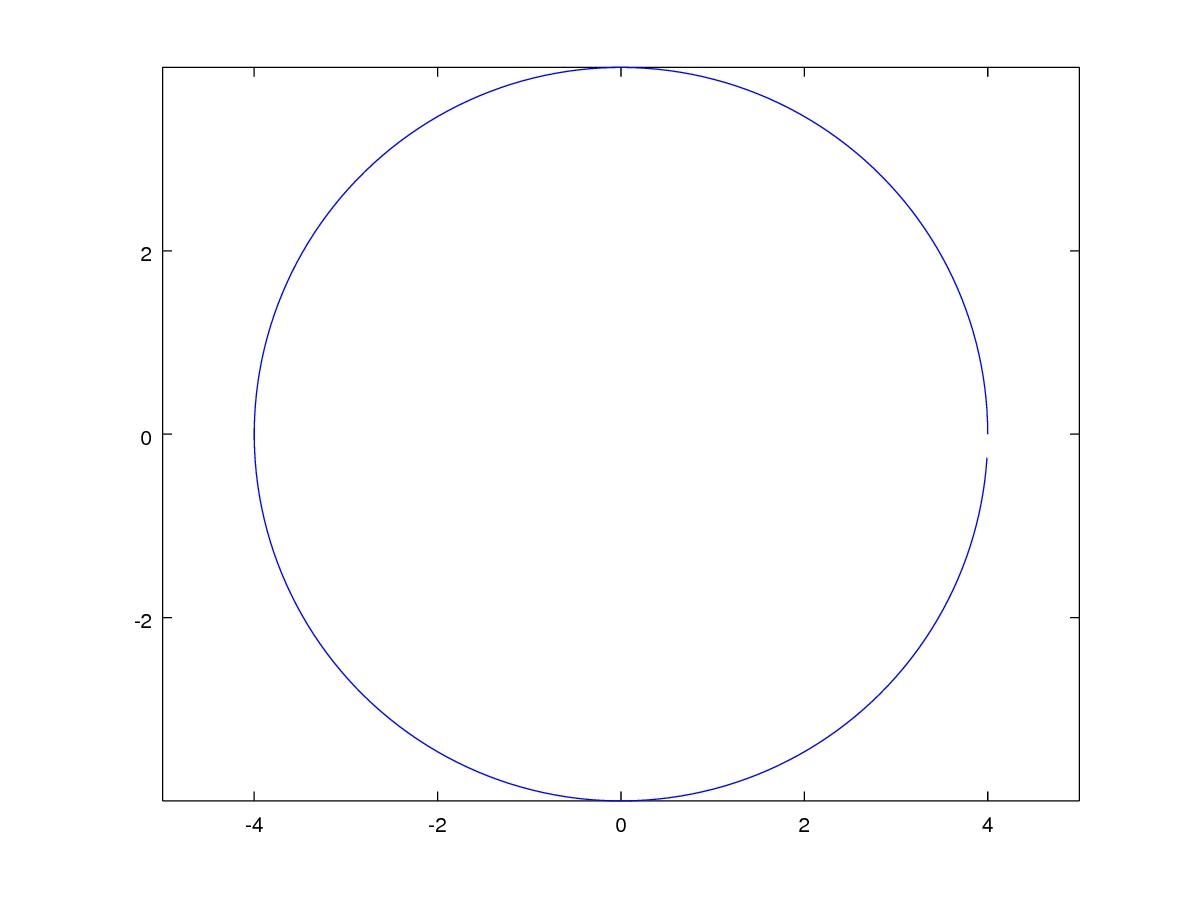
\includegraphics[scale=.3]{../octave/f4.jpg} & 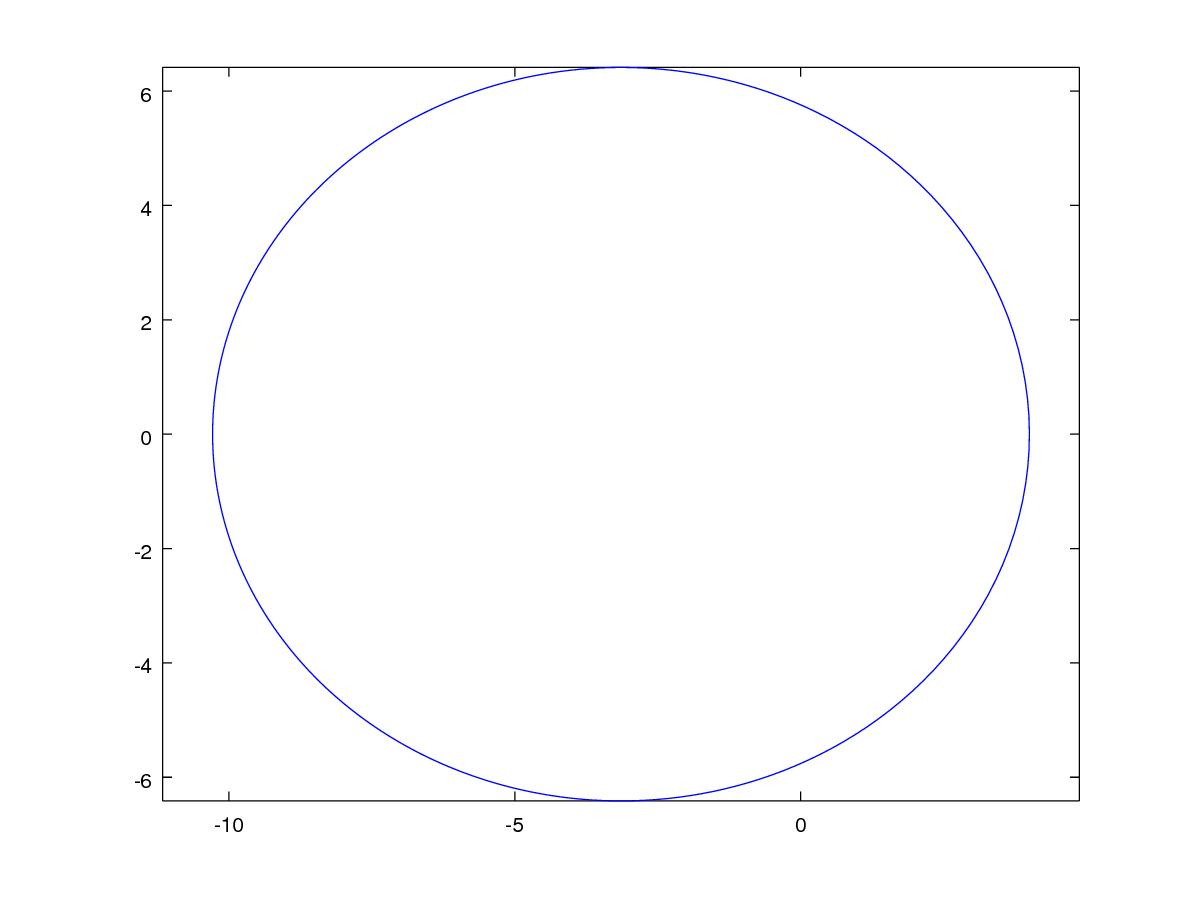
\includegraphics[scale=.3]{../octave/f5.jpg}\\
$[0.8,0.5,200]$ & $[0.4,0.25,35]$\\
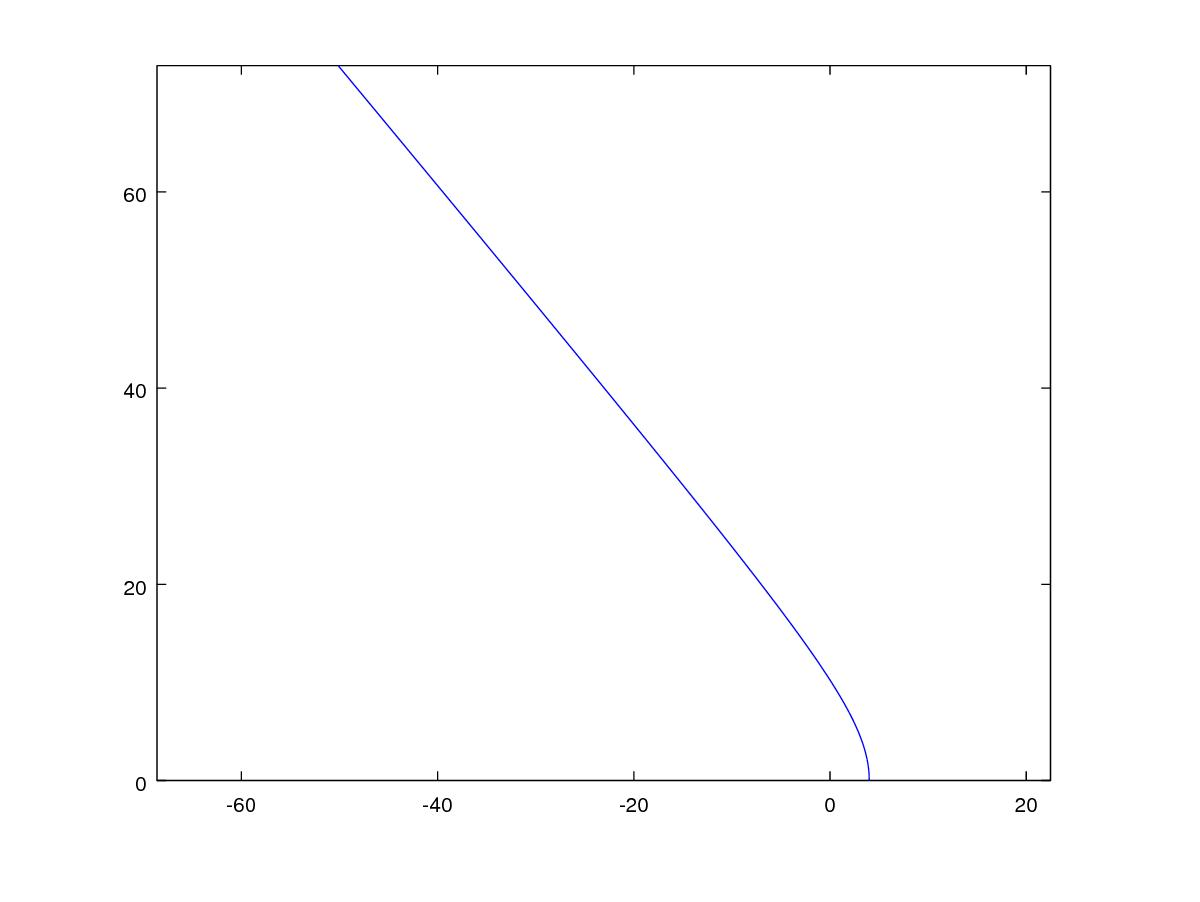
\includegraphics[scale=.3]{../octave/f6.jpg} & 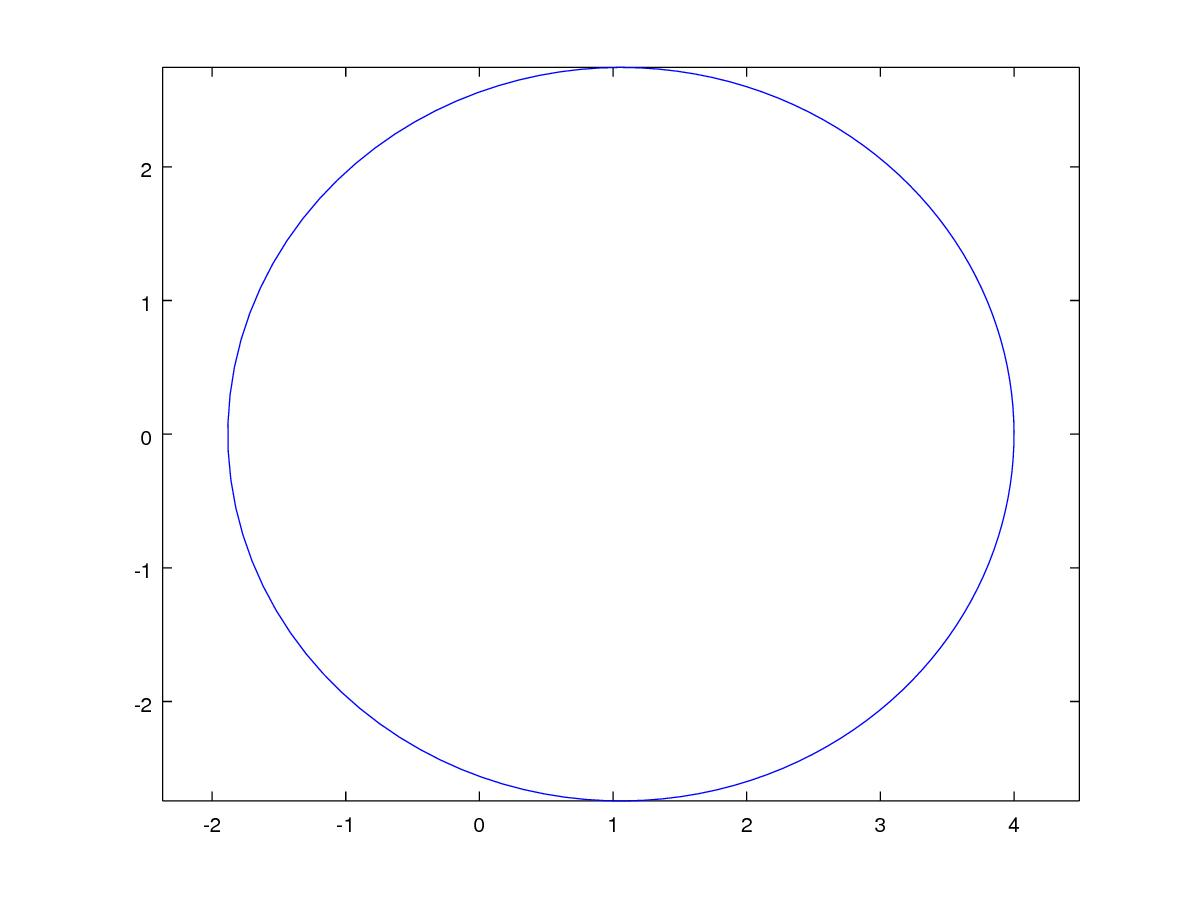
\includegraphics[scale=.3]{../octave/f7.jpg}\\
$[0.2,0.25,30]$ & $[0.2,0.05,30]$\\
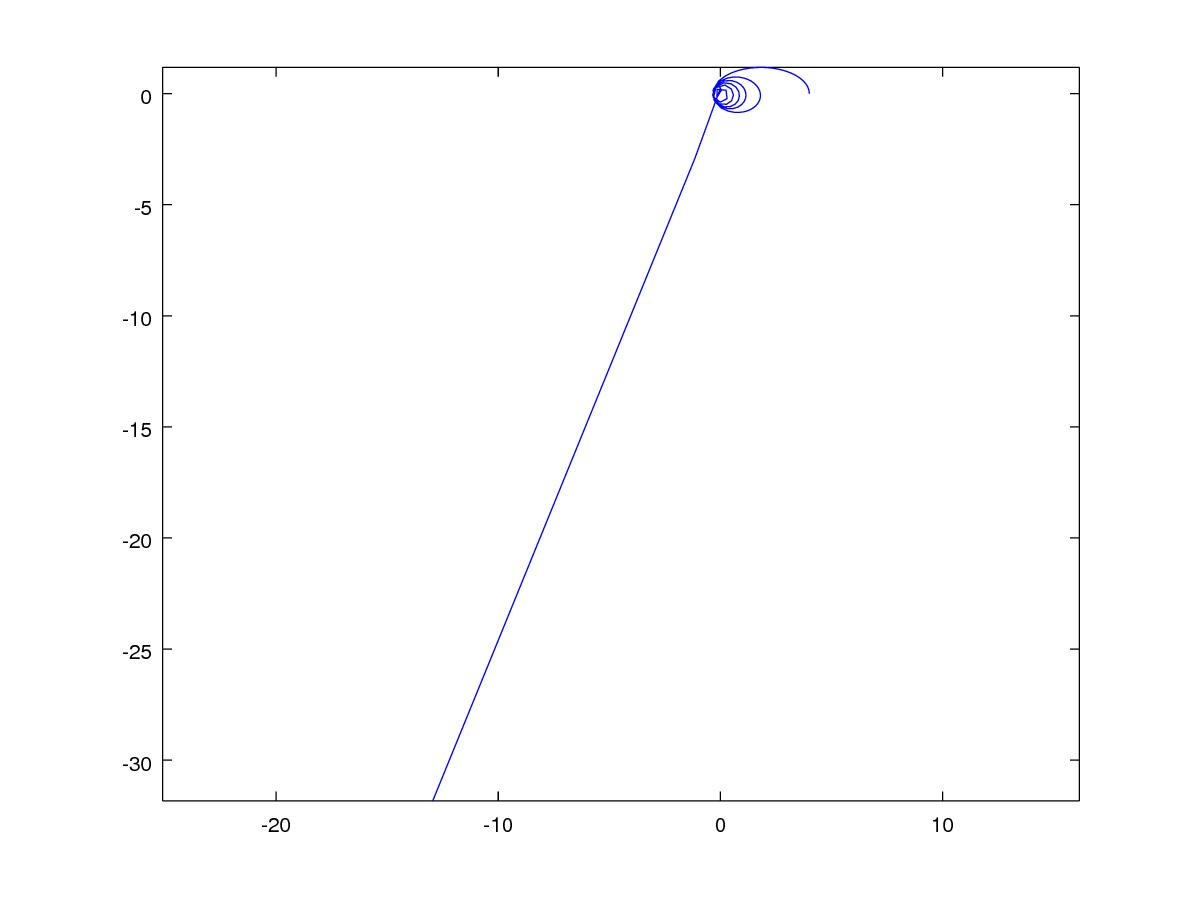
\includegraphics[scale=.3]{../octave/f8.jpg} & 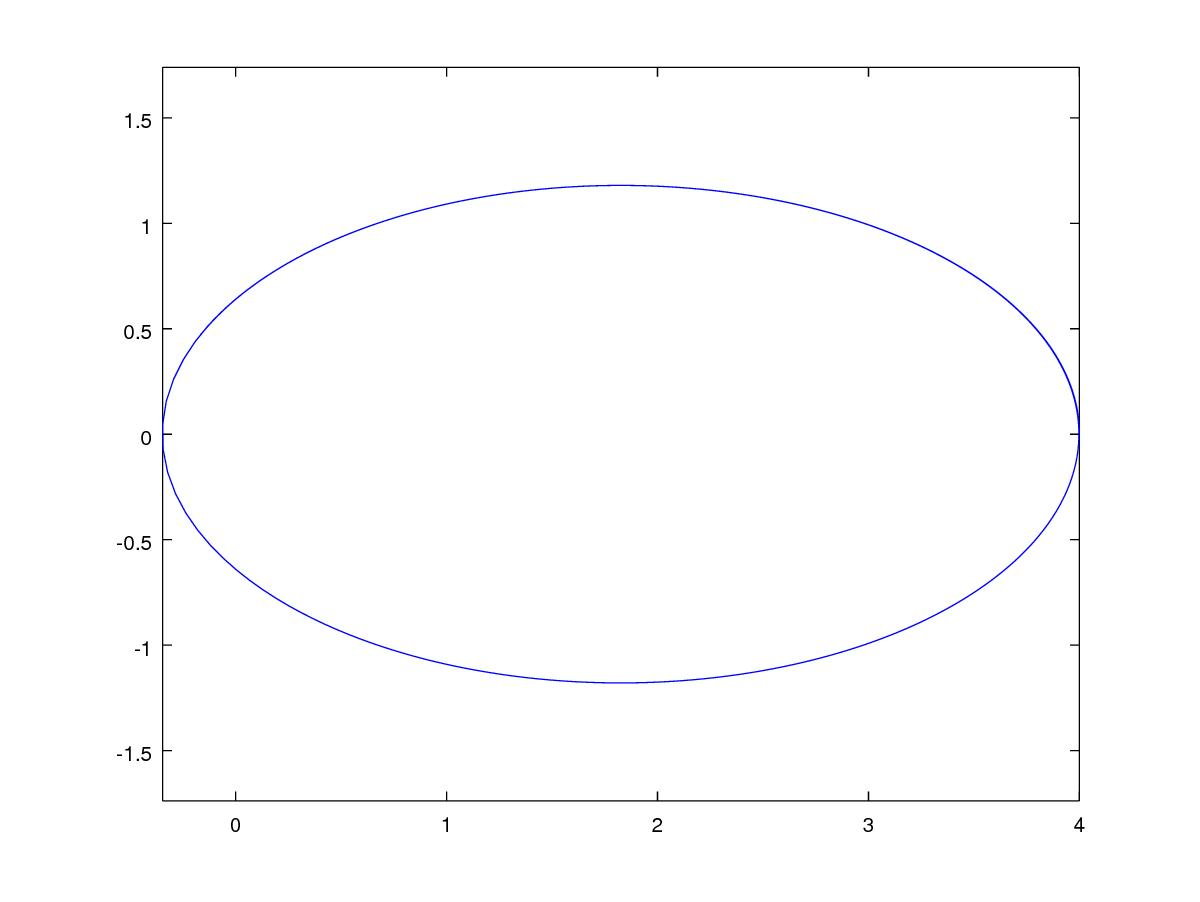
\includegraphics[scale=.3]{../octave/f9.jpg}
\end{tabular}\\
this is my command line
\lstinputlisting{../octave/d3.txt}
\end{enumerate}




\end{document}